\documentclass[12pt,-letter paper]{article}
\usepackage{siunitx}
\usepackage{setspace}
\usepackage{gensymb}
\usepackage{xcolor}
\usepackage{caption}
%\usepackage{subcaption}
\doublespacing
\singlespacing
\usepackage[none]{hyphenat}
\usepackage{amssymb}
\usepackage{relsize}
\usepackage[cmex10]{amsmath}
\usepackage{mathtools}
\usepackage{amsmath}
\usepackage{commath}
\usepackage{amsthm}
\usepackage{graphicx} 
% \usepackage{circuitikz} 
\interdisplaylinepenalty=2500
%\savesymbol{iint}
\usepackage{txfonts}
%\restoresymbol{TXF}{iint}
\usepackage{wasysym}
\usepackage{amsthm}
\usepackage{mathrsfs}
\usepackage{txfonts}
\let\vec\mathbf{}
\usepackage{stfloats}
\usepackage{float}
\usepackage{hyperref}
\usepackage{cite}
\usepackage{cases}
\usepackage{subfig}
%\usepackage{xtab}
\usepackage{longtable}
\usepackage{multirow}
%\usepackage{algorithm}
\usepackage{amssymb}
%\usepackage{algpseudocode}
\usepackage{enumitem}
\usepackage{mathtools}
%\usepackage{eenrc}
\usepackage[framemethod=tikz]{mdframed}
\usepackage{listings}
%\usepackage{listings}
\usepackage[latin1]{inputenc}
%%\usepackage{color}{   
%%\usepackage{lscape}
\usepackage{textcomp}
\usepackage{titling}
\usepackage{hyperref}
% \usepackage{fulbigskip}   
\usepackage{tikz}
% \usepackage{graphicx}
%\usepackage[left=1in, right=2in, top=1in, bottom=1in]{geometry}

\let\vec\mathbf{}
\usepackage{enumitem}
\usepackage{graphicx}
\usepackage{siunitx}
\let\vec\mathbf{}
\usepackage{enumitem}
\usepackage{graphicx}
\usepackage{enumitem}
\usepackage{tfrupee}
\usepackage{amsmath}
\usepackage{amssymb}
\usepackage{tfrupee}
\DeclareMathOperator*{\Res}{Res}
\newtheorem{theorem}{Theorem}[section]
\newtheorem{problem}{Problem}
\newtheorem{proposition}{Proposition}[section]
\newtheorem{lemma}{Lemma}[section]
\newtheorem{corollary}[theorem]{Corollary}
\newtheorem{example}{Example}[section]
\newtheorem{definition}[problem]{Definition}
\newcommand{\BEQA}{\begin{eqnarray}}
\newcommand{\EEQA}{\end{eqnarray}}
\newcommand{\define}{\stackrel{\triangle}{=}}
\theoremstyle{remark}
\newtheorem{rem}{Remark}

\renewcommand{\thefigure}{\theenumi}
\renewcommand{\thetable}{\theenumi}
\providecommand{\pr}[1]{\ensuremath{\Pr\left(#1\right)}}
\providecommand{\prt}[2]{\ensuremath{p_{#1}^{\left(#2\right)} }}        % own macro for this question
\providecommand{\qfunc}[1]{\ensuremath{Q\left(#1\right)}}
\providecommand{\sbrak}[1]{\ensuremath{{}\left[#1\right]}}
\providecommand{\lsbrak}[1]{\ensuremath{{}\left[#1\right.}}
\providecommand{\rsbrak}[1]{\ensuremath{{}\left.#1\right]}}
\providecommand{\brak}[1]{\ensuremath{\left(#1\right)}}
\providecommand{\lbrak}[1]{\ensuremath{\left(#1\right.}}
\providecommand{\rbrak}[1]{\ensuremath{\left.#1\right)}}
\providecommand{\cbrak}[1]{\ensuremath{\left\{#1\right\}}}
\providecommand{\lcbrak}[1]{\ensuremath{\left\{#1\right.}}
\providecommand{\rcbrak}[1]{\ensuremath{\left.#1\right\}}}
\newcommand{\sgn}{\mathop{\mathrm{sgn}}}
\providecommand{\abs}[1]{\left\vert#1\right\vert}
\providecommand{\res}[1]{\Res\displaylimits_{#1}} 
\providecommand{\norm}[1]{\left\lVert#1\right\rVert}
%\providecommand{\norm}[1]{\lVert#1\rVert}
\providecommand{\mtx}[1]{\mathbf{#1}}
\providecommand{\mean}[1]{E\left[ #1 \right]}
\providecommand{\cond}[2]{#1\middle|#2}
\providecommand{\fourier}{\overset{\mathcal{F}}{ \rightleftharpoons}}
%\providecommand{\hilbert}{\overset{\mathcal{H}}{ \rightleftharpoons}}
%\providecommand{\system}{\overset{\mathcal{H}}{ \longleftrightarrow}}
	%\newcommand{\solution}[2]{\textbf{Solution:}{#1}}
\newcommand{\solution}{\noindent \textbf{Solution: }}
\newcommand{\cosec}{\,\text{cosec}\,}
\providecommand{\dec}[2]{\ensuremath{\overset{#1}{\underset{#2}{\gtrless}}}}
\newcommand{\myvec}[1]{\ensuremath{\begin{pmatrix}#1\end{pmatrix}}}
\newcommand{\mydet}[1]{\ensuremath{\begin{vmatrix}#1\end{vmatrix}}}
\providecommand{\rank}{\text{rank}}
\providecommand{\pr}[1]{\ensuremath{\Pr\left(#1\right)}}
\providecommand{\qfunc}[1]{\ensuremath{Q\left(#1\right)}}
	\newcommand*{\permcomb}[4][0mu]{{{}^{#3}\mkern#1#2_{#4}}}
\newcommand*{\perm}[1][-3mu]{\permcomb[#1]{P}}
\newcommand*{\comb}[1][-1mu]{\permcomb[#1]{C}}
\providecommand{\qfunc}[1]{\ensuremath{Q\left(#1\right)}}
\providecommand{\gauss}[2]{\mathcal{N}\ensuremath{\left(#1,#2\right)}}
\providecommand{\diff}[2]{\ensuremath{\dfrac{d{#1}}{d{#2}}}}
\providecommand{\myceil}[1]{\left \lceil #1 \right \rceil }
\newcommand{\sinc}{\,\text{sinc}\,}
\newcommand{\rect}{\,\text{rect}\,}
\newcommand{\E}{\mathbb{E}}
\newcommand{\Var}{\mathrm{Var}}
\begin{document}
\vspace{3cm}
\title{ GATE EE2016, 11}
\author{DHRUV PARASHAR}
\maketitle
\newpage
\bigskip
\renewcommand{\thefigure}{\theenumi}
\renewcommand{\thetable}{\theenumi}
\begin{enumerate}
 \item Consider the following circuit which uses a $2$-to-$1$ multiplexer as shown in the figure below. The Boolean expression for output F in terms of A and B is
\begin{figure}[h!]
		      \begin{center}
			      \tikzset{every picture/.style={line width=0.75pt}} %set default line width to 0.75pt        

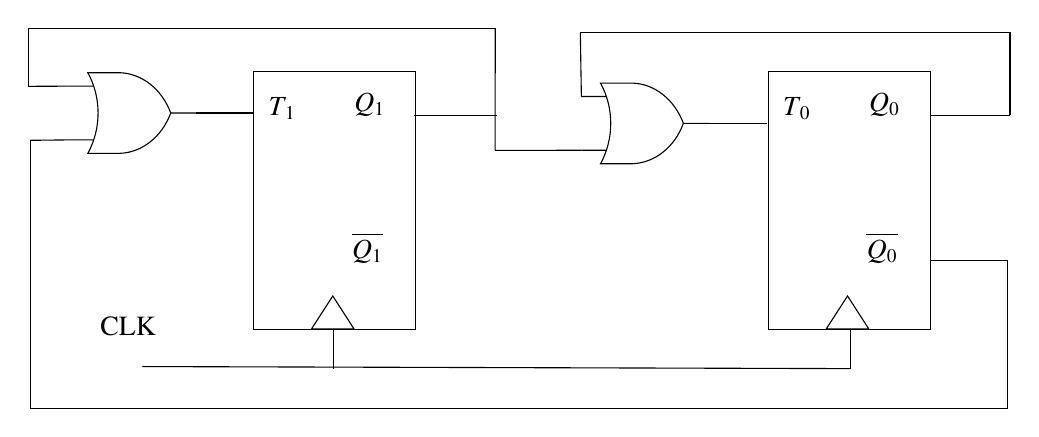
\begin{tikzpicture}[x=0.75pt,y=0.75pt,yscale=-1,xscale=1]
%uncomment if require: \path (0,300); %set diagram left start at 0, and has height of 300

%Shape: Rectangle [id:dp8202540055907639] 
\draw   (158,53) -- (236,53) -- (236,177) -- (158,177) -- cycle ;
%Shape: Or Gate [id:dp08978132180586507] 
\draw   (78.22,53.43) -- (93.58,53.43) .. controls (104.3,53.77) and (113.88,61.34) .. (118.16,72.85) .. controls (113.88,84.36) and (104.3,91.93) .. (93.58,92.28) -- (78.22,92.28) .. controls (84.8,80.25) and (84.8,65.45) .. (78.22,53.43) -- cycle (69,59.9) -- (81.29,59.9) (69,85.8) -- (81.29,85.8) (118.16,72.85) -- (130.45,72.85) ;
%Shape: Triangle [id:dp8379215440652463] 
\draw   (196.23,161) -- (206.45,176.85) -- (186,176.85) -- cycle ;
%Shape: Rectangle [id:dp5064333177931405] 
\draw   (406,53) -- (484,53) -- (484,177) -- (406,177) -- cycle ;
%Shape: Triangle [id:dp04508106309695603] 
\draw   (444.23,161) -- (454.45,176.85) -- (434,176.85) -- cycle ;
%Straight Lines [id:da8430836438701459] 
\draw    (130.45,72.85) -- (158.45,72.85) ;
%Shape: Or Gate [id:dp27911316649955176] 
\draw   (325.22,58.43) -- (340.58,58.43) .. controls (351.3,58.77) and (360.88,66.34) .. (365.16,77.85) .. controls (360.88,89.36) and (351.3,96.93) .. (340.58,97.28) -- (325.22,97.28) .. controls (331.8,85.25) and (331.8,70.45) .. (325.22,58.43) -- cycle (316,64.9) -- (328.29,64.9) (316,90.8) -- (328.29,90.8) (365.16,77.85) -- (377.45,77.85) ;
%Straight Lines [id:da7800420433441013] 
\draw    (377.45,77.85) -- (405.45,77.85) ;
%Straight Lines [id:da7788178738488024] 
\draw    (274.45,90.85) -- (316,90.8) ;
%Straight Lines [id:da39345195977505776] 
\draw    (235.5,74) -- (275.5,74) ;
%Straight Lines [id:da6068351001271327] 
\draw    (274.5,32) -- (274.45,90.85) ;
%Straight Lines [id:da18722802985553144] 
\draw    (49.5,32) -- (274.5,32) ;
%Straight Lines [id:da5744513622437428] 
\draw    (49.5,32) -- (49.5,60) ;
%Straight Lines [id:da80433220708581] 
\draw    (69,59.9) -- (49.5,60) ;
%Straight Lines [id:da6540890230403057] 
\draw    (521.5,144) -- (484.5,144) ;
%Straight Lines [id:da10980162685426853] 
\draw    (521.5,215) -- (521.5,144) ;
%Straight Lines [id:da6573970266628919] 
\draw    (50.5,215) -- (521.5,215) ;
%Straight Lines [id:da8030222177883335] 
\draw    (50.5,215) -- (50.5,86) ;
%Straight Lines [id:da4832475128489785] 
\draw    (50.5,86) -- (69,85.8) ;
%Straight Lines [id:da043356258414056326] 
\draw    (316,64.9) -- (315.5,34) ;
%Straight Lines [id:da6906606003899586] 
\draw    (522.5,34) -- (315.5,34) ;
%Straight Lines [id:da13292875849313357] 
\draw    (522.5,34) -- (522.5,74) ;
%Straight Lines [id:da8943203868157404] 
\draw    (522.5,74) -- (484.5,74) ;
%Straight Lines [id:da13168982284438902] 
\draw    (104.5,195) -- (445.5,196) ;
%Straight Lines [id:da18651973646229014] 
\draw    (196.5,177) -- (196.5,196) ;
%Straight Lines [id:da9854734273448209] 
\draw    (445.5,177) -- (445.5,196) ;

% Text Node
\draw (164,64) node [anchor=north west][inner sep=0.75pt]   [align=left] {$\displaystyle T_{1}$};
% Text Node
\draw (205,62) node [anchor=north west][inner sep=0.75pt]   [align=left] {$\displaystyle Q_{1}$};
% Text Node
\draw (204,129) node [anchor=north west][inner sep=0.75pt]   [align=left] {$\displaystyle \overline{Q_{1}}$};
% Text Node
\draw (412,64) node [anchor=north west][inner sep=0.75pt]   [align=left] {$\displaystyle T_{0}$};
% Text Node
\draw (453,62) node [anchor=north west][inner sep=0.75pt]   [align=left] {$\displaystyle Q_{0}$};
% Text Node
\draw (452,129) node [anchor=north west][inner sep=0.75pt]   [align=left] {$\displaystyle \overline{Q_{0}}$};
% Text Node
\draw (83,170) node [anchor=north west][inner sep=0.75pt]   [align=left] {CLK};


\end{tikzpicture}

			      \caption{}
		      \end{center}
	      \end{figure}
\begin{enumerate}
\item A $\oplus$ B \vspace{3pt}
\item $\overline{\text{A + B}}$ \vspace{3pt}
\item A + B \vspace{3pt}
\item  $\overline{\text{A $\oplus$ B}}$ \vspace{3pt}
\end{enumerate}
\end{enumerate}



\end{document}
